\documentclass[man]{apa6}

\usepackage[american]{babel}

\usepackage{hyperref}

\usepackage{csquotes}
\usepackage[style=apa,sortcites=true,sorting=nyt,backend=biber]{biblatex}
\DeclareLanguageMapping{american}{american-apa}
\addbibresource{bibliography.bib}

\title{System Music With Web Audio API and Machine Learning}
\shorttitle{Final Research Paper}

\author{Nianze Liu}
\affiliation{New York University}

\leftheader{Liu}

\abstract{This article introduces the concept of online system music, which is powered up by Web Audio API and online machine learning techniques that provide new possibilities to create music. Musicians are able to take advantage of Javascript to build a creative and interactive music systems, which is able to run on any smart devices with a browser, leading to a new way to share the music: not by going to the concert, nor listening to a record, but downloading and running a music system itself that generates music on the fly.}

\keywords{Computer Music, Magenta, Online}

\authornote{Nianze Liu, Department of Music and Performing Arts Professions, Music Technology, NYU Steinhardt.

  Correspondence concerning this article should be addressed to Nianze Liu, 
  Department of Music and Performing Arts Professions, Music Technology, 
  NYU Steinhardt, 35 West 4th Street, 10th Floor, New York, NY
  10012.  E-mail: nl1951@nyu.edu}

\begin{document}
\maketitle

Music usually evolves when new technology is available. For example, the tape recorders, as a cutting edge technology in 1950s, have widely changed music industry, not only in how music is distributed and shared, but also how music is produced. Taking use of magnetic tape recorders, and combined with the phase shifting technique, Steve Reich created a famous piece of music called It's Gonna Rain in 1965, which marks the early experiment period in the field of system music. 

According to \textcite{sutherland1994new}, the term system music means "music with sound continua which evolve gradually, often over very long periods of time." Instead of composing and making music directly by the composer, the core concept of system music is to make a system that generates the music. Back in 1960s and 70s, the system might be built using magnetic tape records, loops, delays and synthesizers. Nowadays, thanks to the development of technology, the system might consist of much more powerful technical elements, such as Web Audio and machine learning.

\section{Web Audio API}

Web Audio API, supported by most modern browsers, provides a convenient way to develop music in the browser. To generate audio in the browser, we firstly need to create an audio context, and inside this context, we create source node (such as audio input in the format of mp3, osicllator, or stream input), effects node (such as reverb, filter, panner, and compressor), and destination node (such as system speakers), and link these nodes in sequence, forming an audio graph. This graph structure is similar to the standard music production workflow in modern digital audio workstation(DAW), and could be illustrated in Figure~\ref{fig:Figure1}:

\begin{center}
  \centering
  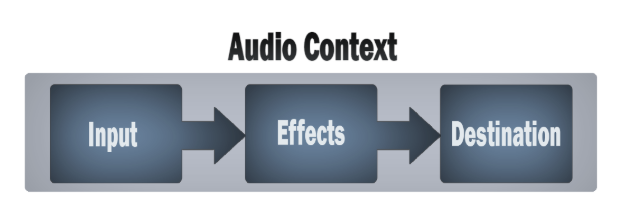
\includegraphics[width=\linewidth]{audio_context.png}
  \captionof{figure}{Web Audio Context Structure}
  \label{fig:Figure1}
\end{center}

With the Web Audio API, we can turn our browser into a simple synthesizer, as mentioned in \textcite{roberts2013web}. I also explored this API by creating an online application that reads in the stock prices in the history and convert the price into beats, which could be found \href{https://nianze.tk/2018/12/use-trading-market-data-to-create-beat-sounds/}{here} to play around, as shown in Figure~\ref{fig:Figure2}. The techniques in this application involve basic use of web audio API and D3.js. All the ticker names are collected from \href{https://dumbstockapi.com/}{dumb stock api}, while all the trading history data comes from \href{https://www.alphavantage.co/}{ALPHA VANTAGE}. 

Currently the mapping from market data to sound is naive:

\begin{enumerate}
  \item Each beat stands for one day of the security price in the past, ordered by the security's trading history
  \item Sound frequency: the higher the daily close price, the higher the frequency
  \item Waveform: if the daily open price is lower than close price, a beat of triangle wave sound is generated, otherwise the sine wave
  \item Duration between each two beats are determined by the earlier day's market volume: larger market volume comes with shorter duration
\end{enumerate}

\begin{center}
  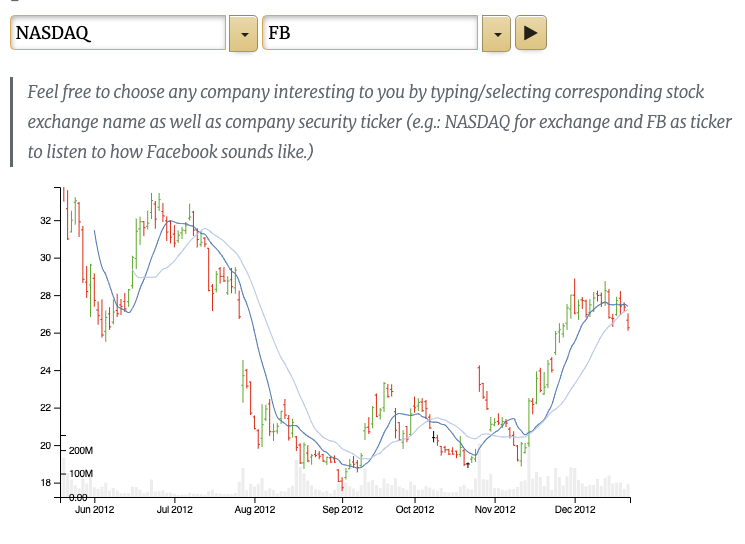
\includegraphics[width=\linewidth]{trade_beats.png}
  \captionof{figure}{Web Audio API Application}
  \label{fig:Figure2}
\end{center}

\section{Machine Learning Toolbox}

Web Audio API alone has already provided us a lot of possibilities to make music in the context of browser, and there are even more powerful tools we can take use of online, such as Magenta.js \parencite{magentajs}, which is a Javascript library providing a lot of powerful machine learning models that can run directly in the browser, without the annoying installation process. Following are a few of these useful machine learning tools.

\subsection{RNN models}
Music is naturally in a sequential structure, which fits well with the structure of recurrent neural network (RNN). RNN has a chain-like loop structure that allows information learned in the previous loop to persist. RNN has shown huge progress in the fields of speech recognition, language modeling, translation and image captioning. Music, if we regart it as some sort of a language in a broader way, might also benefit from the power of RNN.

\subsubsection{Melody RNN}
As mentioned above, this model simply applies the language modeling to melody generation using an LSTM, which is a special form of RNN. The input data format is NoteSequences, which is a data format converted from input MIDI files with pitch range [48,84]. To make the model more powerful so that melodies across a few measures with a larger arch can be caught, some optional optimization techniques such as attention and lookback is also presented.

\subsubsection{Improv RNN}
Similar to the Melody RNN above, the Improv RNN generates monophonic melodies using LSTM structure, except that Improv RNN also reads the underlying chord progression as well as current chord as input, and the inpurt data format is not MIDI but MusicXML.

\subsubsection{Drums RNN}
This model is also using language modeling with an LSTM, targeting the drum track generation. Different from melodies, drum tracks are not monophonic but polyphonic, since there might be multiple drums hit simultaneously. However, since possible combination of different drums hit at the same time is limited, the Drums RNN still represents the different events by a single value. For example, for a drum kit consisting of 9 pieces (bass drum, snare drum, closed and open hi-hat, three toms, and crash and ride cymbals), we only need to use a 512 dimentional one-hot vector to represent all the possible combinations of different drum hit situation, since ${2}^{9}=512$.

\subsubsection{Performance RNN}
This model is an LSTM-based recurrent meural network that tries to catch the style of polyphonic music with their timing and dynamics, as mentioned in \textcite{performance-rnn-2017}. This model is trained on the Yamaha e-Piano Competition dataset, which is a dataset collected from human performance and consists velocities information. The input data event is similar to MIDI, which is defined as a 388 dimensional vector consists of 128 note-on, 128 note-off, 100 time-shift, and 32 velocity events. With good data source, the model is able to output good piece of polyphonic piano pieces in a short period of time, but still lack the overall coherance in the long run.

\subsection{Latent space models}
Except from the RNN modelings, another powerful tool in machine learning is to model the target in latent space. The idea behind latent space modeling is to represent the target dataset originally in a high-dimention by a lower-dimentional latent space code, and we can then apply manipulations to the lower-dimentional representation. An ideal latent space representation should have following properties:

\begin{enumerate}
  \item Expression: any real example can be mapped to some point in the latent space and reconstructed from it.
  \item Realism: any latent space representation corresponds to some realistic examples in original space, including ones not in the training set.
  \item Soothness: nearby points in latent space have similar qualitiesto one another.
\end{enumerate}

Following are two latent space models provided in Magenta.js:

\subsubsection{NSynth}
NSynth \parencite{engel2017neural} tries to model the timbre information and represent them in latent space. The latent space code in NSynth is a 16-dimension temporal embeddings vector. We can apply timestretching, interpolation, and composition to different latent space vectors to create new sound effects different from how we can get from the traditional synthesizers. For example, by adding two temporal embeddings together, say a vector representing the sound of a flute and another one representing the sound of a dog barking, the result is a single merged sound that lies between the two source in a very unique way. One weakness of Nsynth, however, is that it lacks the property of realism.

\subsubsection{MusicVAE}
MusicVAE \parencite{roberts2018hierarchical} is a hierarchical recurrent variational autoencoder that tries to learn the music scores in latent spaces. By using what is called a variational loss technique, instead of limiting the dimensions of the vector to 16 like NSynth, the encoder can produce latent codes with a predefined structure such as from a \href{https://en.wikipedia.org/wiki/Multivariate_normal_distribution}{multivariate normal distribution}, and by constructing new codes with this structure, the property of realistic is ensured. What's more, MusicVAE adopts a noval hierarchical decoder structure that is capable of generating long-term structure from individual latent codes, as shown in Figure~\ref{fig:Figure3}. Thus, given a few input melody example MusicVAE is able to generate a palette of possible melodies that blend those input, similar as how a painter blends and explores color options by mixing and blending different basic colors.

\begin{center}
  \centering
  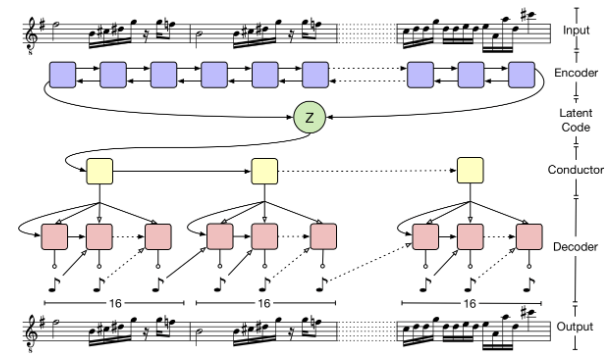
\includegraphics[width=\linewidth]{music_vae.png}
  \captionof{figure}{Structure of MusicVAE}
  \label{fig:Figure3}
\end{center}

\section{Future and Challenges}
As a universal medium available to everyone, internet becomes more powerful thanks to the tools mentioned above, and we can imagine online system music can grow more powerful. For example, web page presents us a canvas that we can naturally use to build interactive systems that combine the audio with visual elements, which connects the composer and the listener in a more interactive way and in some sense, we can say that the listener help generate the music pieces in this interactive system. Moreover, broader application of system music could be achieved by the help of Internet of Things: with the input signals from smart home devices such as Google Home and Amazon Alexa, or biological signals from wearable smart devices such as Apple Watch and Fitbit tracker, online music system can be aware of the environmental context and user state, and generate more adaptive music.

However, we should also be aware of the possible challenges. First of all, all the machine learning models listed above are still too technical for real musicians to take use of. The model output is usually not straightforward or predictable, sometimes leading to confusions. The configurable parameters for these models are still not easy to control. For example, in Performance RNN, we can only use a parameter called temperature (which defaults to 1) to determine the randomness of the output musical piece. This unpredictability will be a bottleneck to create future music, and new models with new structures might need to developed to overcome these difficulties.

\printbibliography

\end{document}